\section{Esercizio 3}
\textit{\textbf{Descrizione:} Eseguire il seguente script Matlab e spiegare i risultati ottenuti:
\newline\newline		
format long e\newline
n=75;\newline
u=1e-300; for i=1:n, u=u*2; end, for i=1:n, u=u/2; end, u\newline
u=1e-300; for i=1:n, u=u/2; end, for i=1:n, u=u*2; end, u}\newline

\noindent \textit{\textbf{Svolgimento:}}\newline

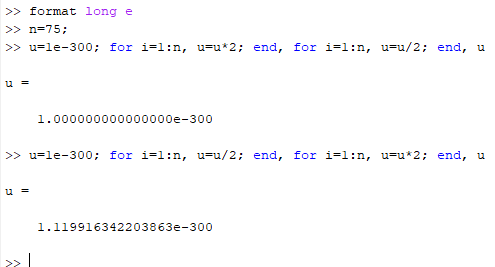
\includegraphics[width=1\linewidth]{img/ex3}
\\~\\
\noindent  in questo script Matlab viene moltiplicato per 2 un valore u=1e-300 per 75 volte, successivamente questo valore u viene diviso per 2 per 75 volte e infine si visualizza il valore in u, poi, viene riportato u al valore di partenza, cio\'e u=1e-300, e viene prima diviso per 2 per 75 volte, poi moltiplicato per 2 per 75 volte  e infine si visualizza il valore in u.
\\~\\
\noindent Se fossimo in matematica esatta, in entrambi i casi, avremmo u che sarebbe uguale al valore di partenza poich\'e \'e stato prima moltiplicato e diviso per la stessa cifra ($2^{75}$) e poi diviso e moltiplicato per la stessa cifra ($2^{75}$). Tuttavia in Matlab i calcoli vengono effettuati in matematica finita e pertanto nel primo caso, in cui la moltiplicazione precede la divisione otteniamo lo stesso risultato che otterremmo in matematica esatta ovvero \text{1.000000000000000e-300}, nel secondo caso invece otteniamo un valore differente ovvero \text{1.119916342203863e-300}.
\\~\\
\noindent La causa per cui nel secondo caso otteniamo un valore diverso da quello iniziale \'e da attribuire ad un errore di round-off, per la precisione un errore di underflow, causato nel primo ciclo in cui viene u viene diviso per 2 per 75 volte, dove, durante una delle iterzioni viene a verificarsi che, $0 < \left | u \right |< r_{min}$ . Essendo che $ r_{min}$ \'e il pi\'u piccolo numero di macchina diverso da zero rappresentabile in valore assoluto, il valore di u viene arrotondato a questo, generando cos\'i un errore di underflow .
\newline
\newline